\chapter{Method}

\section{Detailed Problem}

\paragraph*{}
When people interact with their bank or hospital through online services accessed from a personal computer or a smartphone, they expect their data is secure. In other words: confidentiality, integrity, and authenticity are guaranteed. On a personal computer, these requirements have become evident, and many technologies for cyber security exist \cite{RajasekharaiahK.M2020CSCa}, \cite{LakhdharYosra2021PSfS}. The problem with systems like smartphones and IoT devices is that their hardware is not as extensive as that of a personal computer, making many of these technologies unfeasible. So, while people often have the same expectations towards security, in both cases this is still a challenge when it comes to smartphones. Therefore, the security of a system like a smartphone is very crucial because lots of people are unaware of the possible threats they face.

\paragraph*{}
Adversaries have many possibilities when it comes to stealing sensitive data from smartphone users while the data is being used during execution or stored on the device. \cite{JavedAbdulRehman2020Adms} for instance, propose AlphaLogger, which infers the letters being typed on a soft keyboard based on the vibrations, and \cite{SongWenna2020ADAv} were able to achieve identity theft through data cloning of auto-login credentials. Besides custom attacks, there are plenty of well-known risks as well. \cite{SetyawanRico2020Abro} have executed a review of various malicious software threats and mitigations, \cite{GRAVELLIERJoseph2021RHAo} researched software attacks that take advantage of hardware resources to conduct fault injection or side-channel analysis, and \cite{KumarSudesh2020AoAS} reviewed the possible threats that can be introduced by smartphone providers altering the Android OS to add their signature flavor. These attacks are possible due to smartphones being inferior to personal computers in terms of hardware. As similarly to IoT devices, a lot of focus lies on the performance of the final product. This performance is often hard to achieve because the resources want to be kept to a minimum to lower the price or keep the device small. Security is still seen as a performance killer, which is very unfortunate because it should play an essential role in the design and implementation of a system. 

\section{System Model}

\begin{figure}[h]
\centering
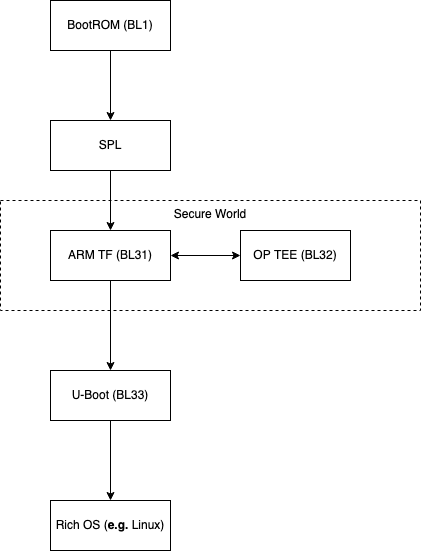
\includegraphics[width=0.5\textwidth]{boot_flow}
\caption{PineA64 boot flow for OP-TEE and Linux}
\caption*{Source: \cite{blog}}
\label{boot}
\end{figure}

\paragraph*{}
The system model used in this thesis is an open system. With an open system, we mean that the owner is not constrained by any means to how they desire to use their device. These restrictions can go from limitations on what software can run on the device, to certain functions that cannot be controlled by the user in any way. The openness discussed here is not the same as open-source systems, but it shares many properties. In an open-source system, all the stakeholders of the system can inspect every detail about the system they want. Using this technique the stakeholders can gain lots of knowledge about the system, which could facilitate interoperability with certain software or devices. The stakeholders could also gain confidence in the qualities and capacities of the system if they can investigate these details. This is the type of confidence and understanding our open system should also provide, but it is mainly focused on not constraining the owner in their capabilities while using the device.

\paragraph*{}
The concrete system is a smartphone that is owned by a user but for which multiple software providers offer applications. These providers don't necessarily trust each other but they do want guarantees that the execution of their software will not be interfered with by software of other providers. The user of the device is also its owner, with full control over what software can be installed and run on the platform. In an open system like the PinePhone, these values are pursued to minimize the constraints the user experiences while using his device. This is very different from large smartphone companies where the company has a signature key which is kept secret. Programs that are not signed with this signature key will be rejected for installation on the device. 

\paragraph*{}
The smartphone, in this case, is a PinePhone which is equipped with 4 ARM Cortex A53 Cores that are TrustZone enabled. Lots of smartphones have ARM processors as SoC, which means that ARM TrustZone is the ideal candidate for the implementation. For this TEE to work correctly, a trusted kernel is required. OP-TEE is used, which provides the interfaces to communicate with the TEE and call TAs from the NW. The NW runs a Mobian Linux distribution as kernel which is specifically written for smartphone devices. The system can be put together as described in \cite{blog}, and shown in figure \ref{boot} using the source of the Mobian distribution \cite{mobian}, OP-TEE \cite{OPTEEgit}, U-boot \cite{u-boot} and the ARM Trusted Firmware \cite{ARMfirmware}. Unfortunately, this was not realized in this thesis, so the QEMU emulator \cite{QEMU} was used to test the code and run the experiments. QEMU allows running OP-TEE on a desktop while emulating the TEE. Because OP-TEE can run on the PinePhone, the code and experiments should be reproducible on the PinePhone if correctly configured with OP-TEE.

\section{Attacker Model}

\paragraph*{}
The adversary we are trying to protect against intends to get access to sensitive data from the device or execute arbitrary code on the device. By achieving this, he could abuse the personal information of the victim or his hardware respectively. The attacker is assumed to have physical access to the device, which could be achieved by stealing the device or through the evil maid attack, where the device is unattended during a period of time and the attacker has temporary physical access to it. He could also launch OS attacks which means he exploits a security vulnerability in the rich OS, which allows him to take control of it and with this control try to maliciously modify other parts of the system. Exploiting a security vulnerability inside the OS and taking control over it by itself, is also undesirable behavior. Lastly, the attacker can execute software attacks which comprise insertion of malware, tampering with the control flow of executing processes, and so on. The attacker is not able to break encryption algorithms deemed to be secure by the literature and cannot violate the security guarantees a TEE provides.

\paragraph*{}
Physical access brings along lots of risks because the adversary has a variety of possible attacks he could launch from this position. The TEE can, when combined with some specific hardware, make these attacks ineffective or a lot harder to execute. For instance, reading from the hardware memory becomes infeasible because everything on there that is sensitive is encrypted by the TEE. Only the TEE can decrypt this information. The decryption key is stored in a secure key store or a TPM or can be derived from the RoT. Tampering with memory can be prevented by using secure boot. It ensures that the TEE is started up in a secure and known state from which a trusted base can be ensured. With this trusted base, attestation could be run on the memory to check whether inconsistent memory pages can be found before they receive control in case they are code pages. Another hardware attack is one where a physical back door is exploited. This is assumed to be impossible because the processor has been designed for security purposes and thus no back doors should be available. The main advantage defenders have in terms of hardware attacks, is that they are often very hard to execute. There are still lots of hardware attacks for which TEEs are vulnerable: manipulation of RAM and eFuse bypassing secure boot \cite{GrossMathieu2021BTmi}, micro-architectural structures leaking information \cite{RyanKeegan2019HHEE}, and electromagnetic analysis of side-channels \cite{BukasaSebanjilaKevin2018HTCB}. These attacks are very advanced and would be hard to execute, which is the reason why they are not taken into account in this thesis.

\paragraph*{}
OS/Firmware attacks can compromise all user-level applications because the OS is the trusted layer on which these user-level applications rely. This is the main area where ARM TrustZone and other TEE implementations make a very big difference in security. ARM TrustZone, for instance, is implemented below the rich OS, which means that the trusted kernel has more privileges than the latter. The rich OS has of course more functionality, but to achieve this functionality, it will in some cases rely on the trusted kernel. In case an OS attack has succeeded, a TEE increases the security by shielding the user-level applications from this OS. This is done by allowing the user-level application to request services like trusted I/O and secure memory from the TEE itself, without interference from the OS. Examples of this are a container using ARM TrustZone \cite{HuaZhichao2021Tpcf}, securing camera and location peripherals \cite{SalmanAmmarS2021SMSG}, and checking whether the OS executes system services correctly \cite{GuanLe2017TSEo}. It does not make claims about preventing OS attacks, because the vulnerabilities in the rich OS are still present. The NW could be attested which would allow the detection of an OS attack, but the TEE doesn't have special protection mechanisms to avoid it from happening. This is not surprising of course, since OS attacks are often a consequence of software bugs in the implementation that give rise to security vulnerabilities. These bugs are very hard to avoid due to the large number of lines of code in these rich OS implementations.

\paragraph*{}
Software attacks try to tamper with the control flow of certain program executions, or get hold of sensitive data through malicious code. Most of these attacks can be defended against by a TEE implementation, or with the help of a TEE. Applications can be isolated from each other, making it a lot more difficult for a malicious application to tamper with the execution or data of another one. This isolation can be enforced using virtualization or specialized TAs, making sure the application can only be interacted with, using a very well-defined interface. The virtualization needs to be implemented correctly to make sure no data is leaked in between the partitions. In the case of the TA, it can use the TEE functionality to store its data securely. Software attack defense mechanisms based on ARM TrustZone come in many forms, isolate application and secure communication \cite{ZhangDiming2020iIfs}, control flow integrity scheme \cite{KawadaTomoaki2020TRCI}, and reverse engineering protection \cite{BenYehudaRaz2019Pare}.

\section{Solution}

\paragraph*{}
First things first: to make sure the TEE can provide the security it guarantees, it needs to be started up using secure boot. This ensures that the device starts in a known secure state, which can therefore be trusted. To achieve this, a RoT is needed from which a CoT can be constructed. The RoT is often implemented by using a TPM along with hardware memory specifically designed for secure storage, for instance, an eFuse or OCROM. As discussed in \cite{RoT} the PinePhone provides write-once memory in which the hash of a public key can be placed. This key can be used to serve as RoT during trusted boot on the device. Depending on how this memory is used, a discussion about \textit{\enquote{What can be used as a RoT in such an open system?}} can be had. 

\paragraph*{}
When the RoT and subsequently the trusted boot are taken care of, we need to utilize the TEE to improve the security of the smartphone. The ultimate goal would be to guarantee the integrity of the control flow, code, and data on the device, which is a very strict requirement. An achievable target would be to detect violations to this integrity. Attestation can be used to check the integrity of an application or a running system depending on what properties are looked at to measure the reliability of the target. RA is not logical in the context of a smartphone, but the user (who in our case is seen as the owner of the device) could be alerted about the integrity checks. This train of thought will be followed and partially implemented to attempt to answer the question \textit{\enquote{Can attestation be used to increase the security of an open platform without disrupting the openness of the system?}}.

\paragraph*{}
The user plays a critical role in this solution. This is due to the requirement that the device should be secure while the user stays in control. The user can decide which software he considers secure and allow to run on his device. On the other hand, the software providers do not want another process to interfere with the execution control flow of their programs. This can be achieved by having the attestation process run within the TEE on the device, making it tamper-proof against software and OS attacks. The interests of all parties need to be taken into account during the evaluation of the solution to be able to answer the question \textit{\enquote{Does this security solution meet the expectations of all smartphone stakeholders?}}. 

\paragraph*{}
Ensuring the openness of the system is not violated by the proposed security solution, has consequences on the achieved results. These consequences are thoroughly looked at during a comparison with similar security approaches that do not take into account the openness of the system. Besides these comparisons, also possible extensions are discussed that have been implemented by other work but don't require the system to be closed, so these could also be seen as directions for future work. These comparisons attempt to answer the question \textit{\enquote{How does this type of security solution compare with the ones in closed systems?}}